\documentclass{article}
\usepackage{enumerate}
\usepackage{amsmath}
\usepackage{amssymb}
\usepackage{graphicx}
\usepackage{subfigure}
\usepackage{geometry}
\usepackage{caption}
\usepackage{indentfirst}

\usepackage{algorithm}  
\usepackage{algorithmicx}  
\usepackage{algpseudocode}
\renewcommand{\algorithmicrequire}{\textbf{Input:}}  
\renewcommand{\algorithmicensure}{\textbf{Output:}}  
\usepackage{minted}
\usemintedstyle{autumn}
\setminted{linenos,breaklines,tabsize=4,xleftmargin=1.5em}

\geometry{left=3.0cm,right=3.0cm,top=3.0cm,bottom=4.0cm}

\title{VE281 Project One Report}
\author{Liu Yihao 515370910207}
\date{}

\begin{document}
\maketitle

\section{Introduction}

In order to study the performances of these six sorting algorithms, I generated different size of arrays and compared the running speed of them (including the std::sort function in STL). Since it's a waste of time to wrote a comparison script written in C++, I chose node-gyp to build the sorting algorithm into a C++ addon of node, and then wrote some Javascript code to benchmark them. Small size of arrays were run for several times so that the result can be more accurate.

\section{Comparison of algorithms}

The limitation of runtime was set to 1s for all algorithms, so some meaningless and slow running were dropped (eg. large array size for bubble sort). Then I used MATLAB to plot two graphs, one of small test cases, and another of all cases.

\subsection{General analysis}

\begin{figure}[!htbp]
\centering
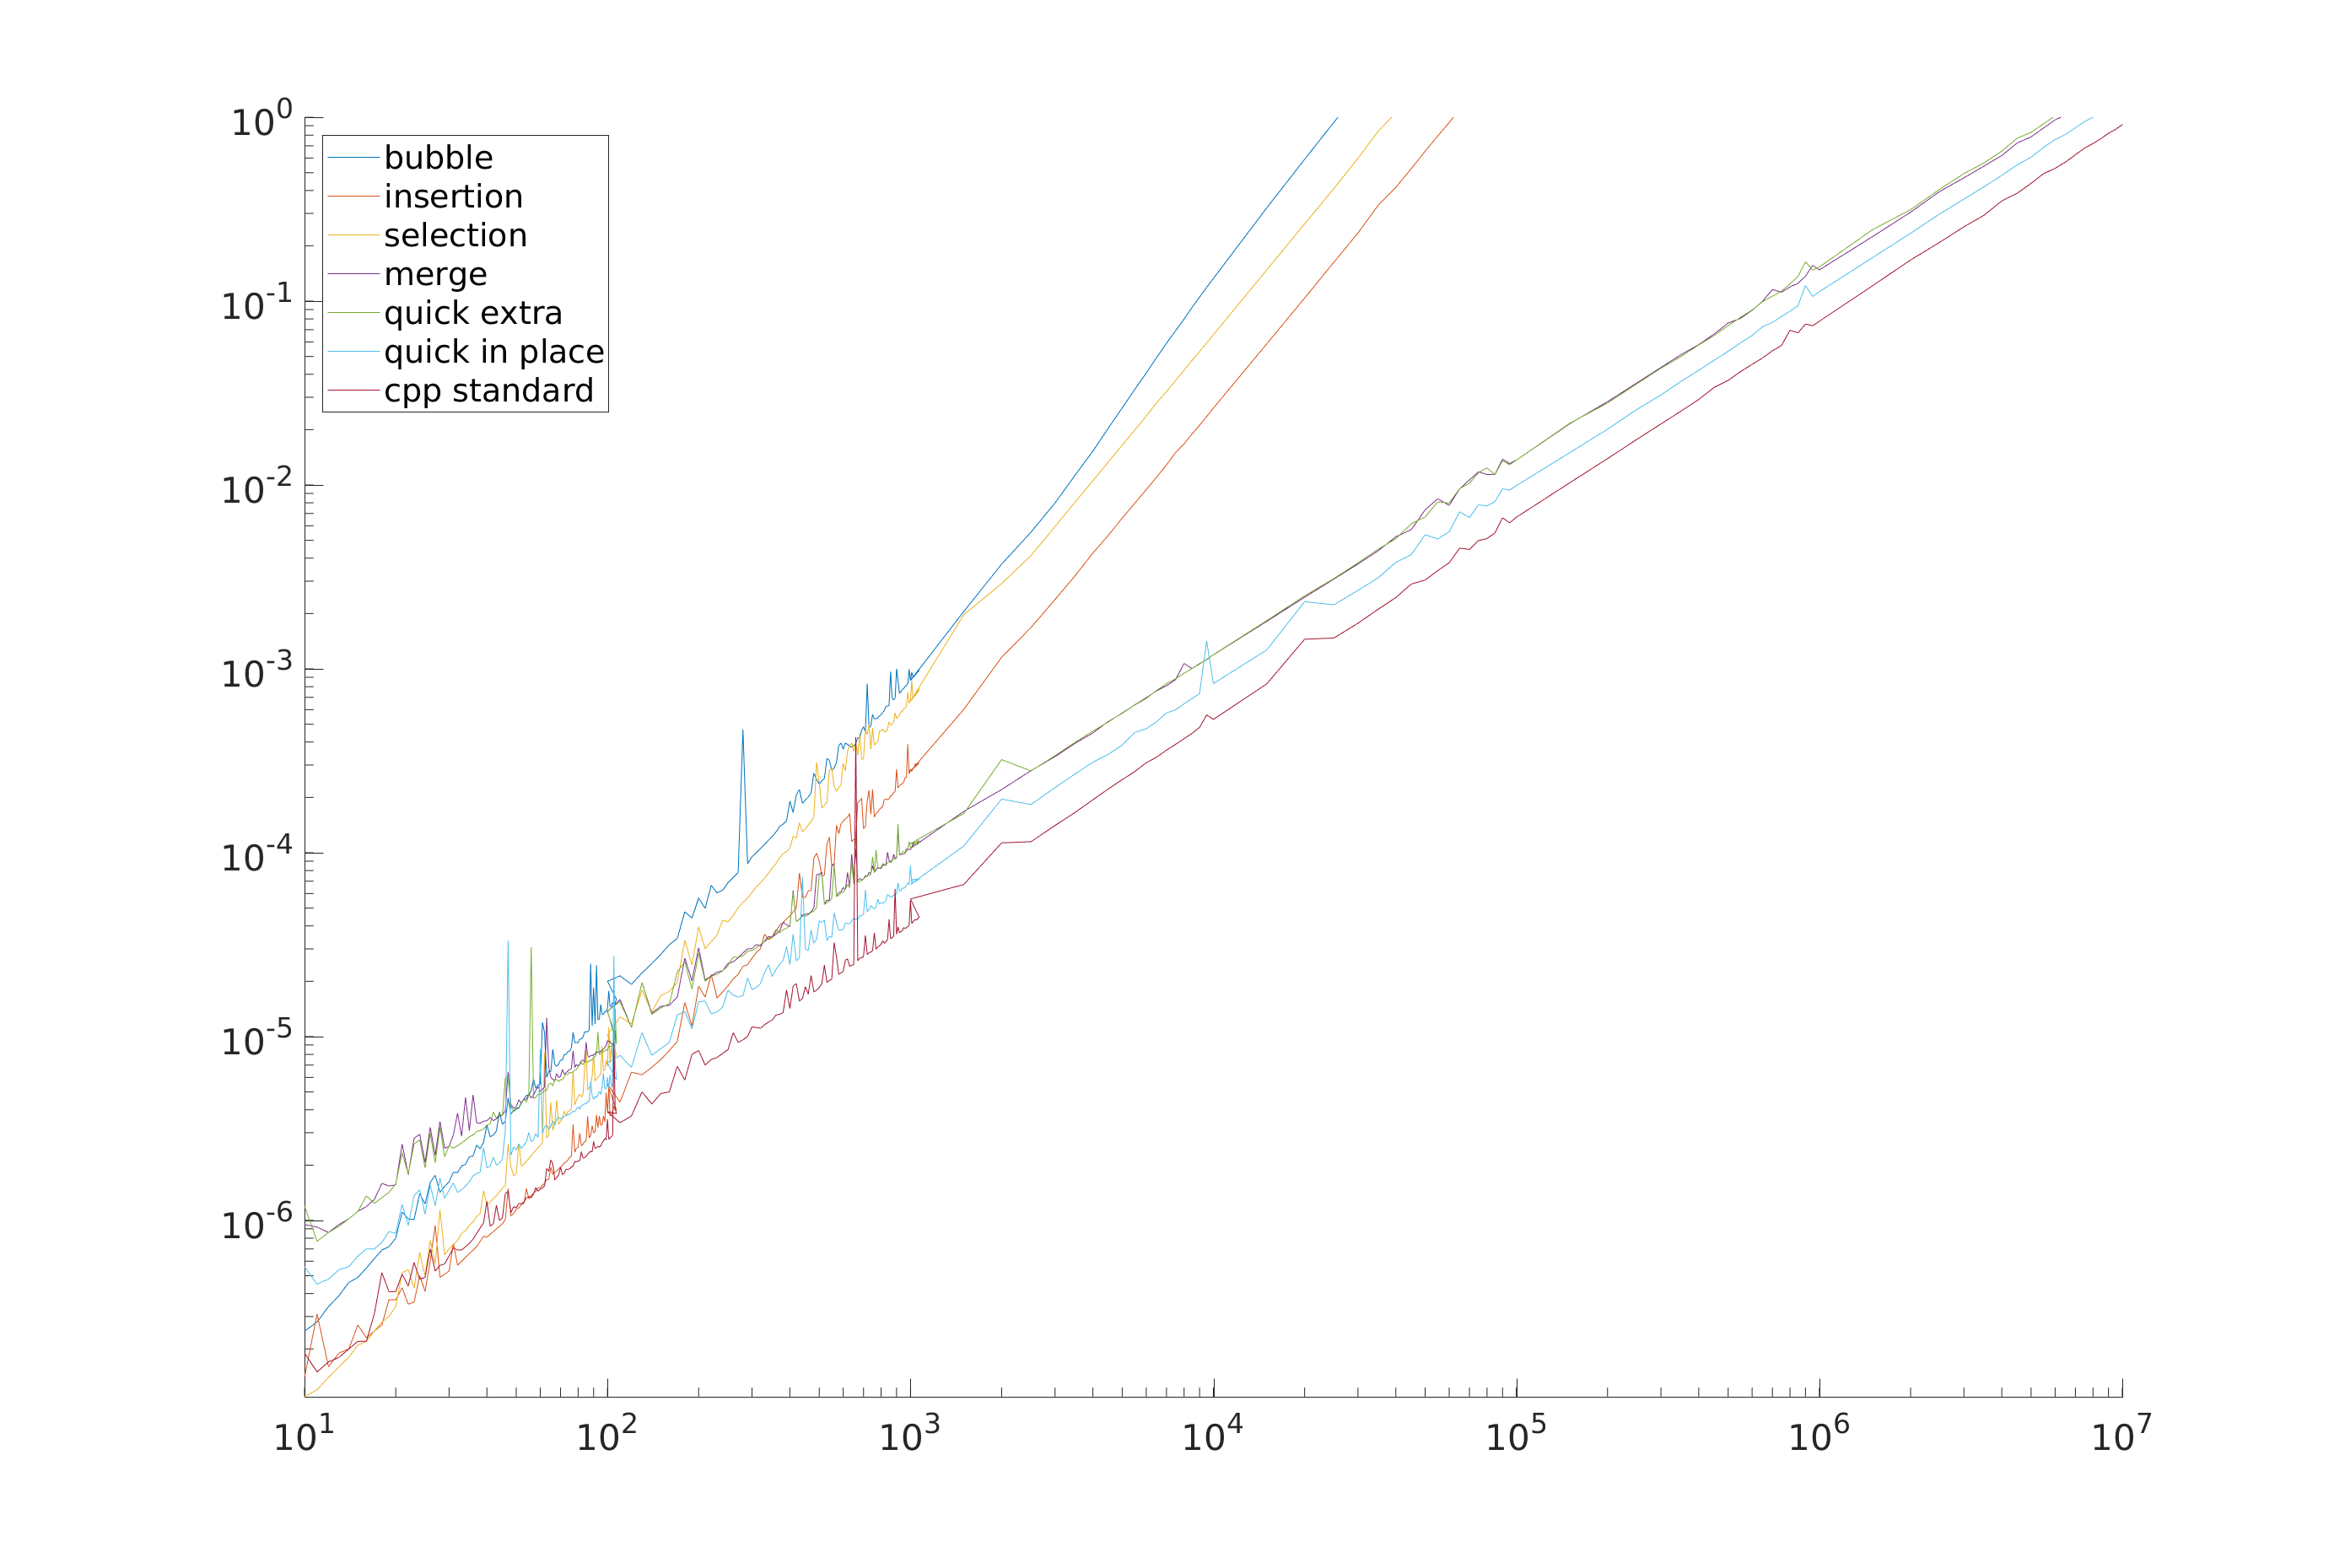
\includegraphics[width=0.8\linewidth]{../benchmark/fig1.png}
\caption{All cases}
\label{fig-1}
\end{figure}

From Figure \ref{fig-1}, we can find that bubble sort, insertion sort and selection sort have the similar running speed, while merge sort and quick sort are also similar on running speed, but faster. The result satisfy the theory that bubble sort, insertion sort and selection sort have time complexity of $O(n^2)$, while merge sort and quick sort have time complexity of $O(n\log n)$.

\subsection{Small data analysis}

\begin{figure}[!htbp]
\centering
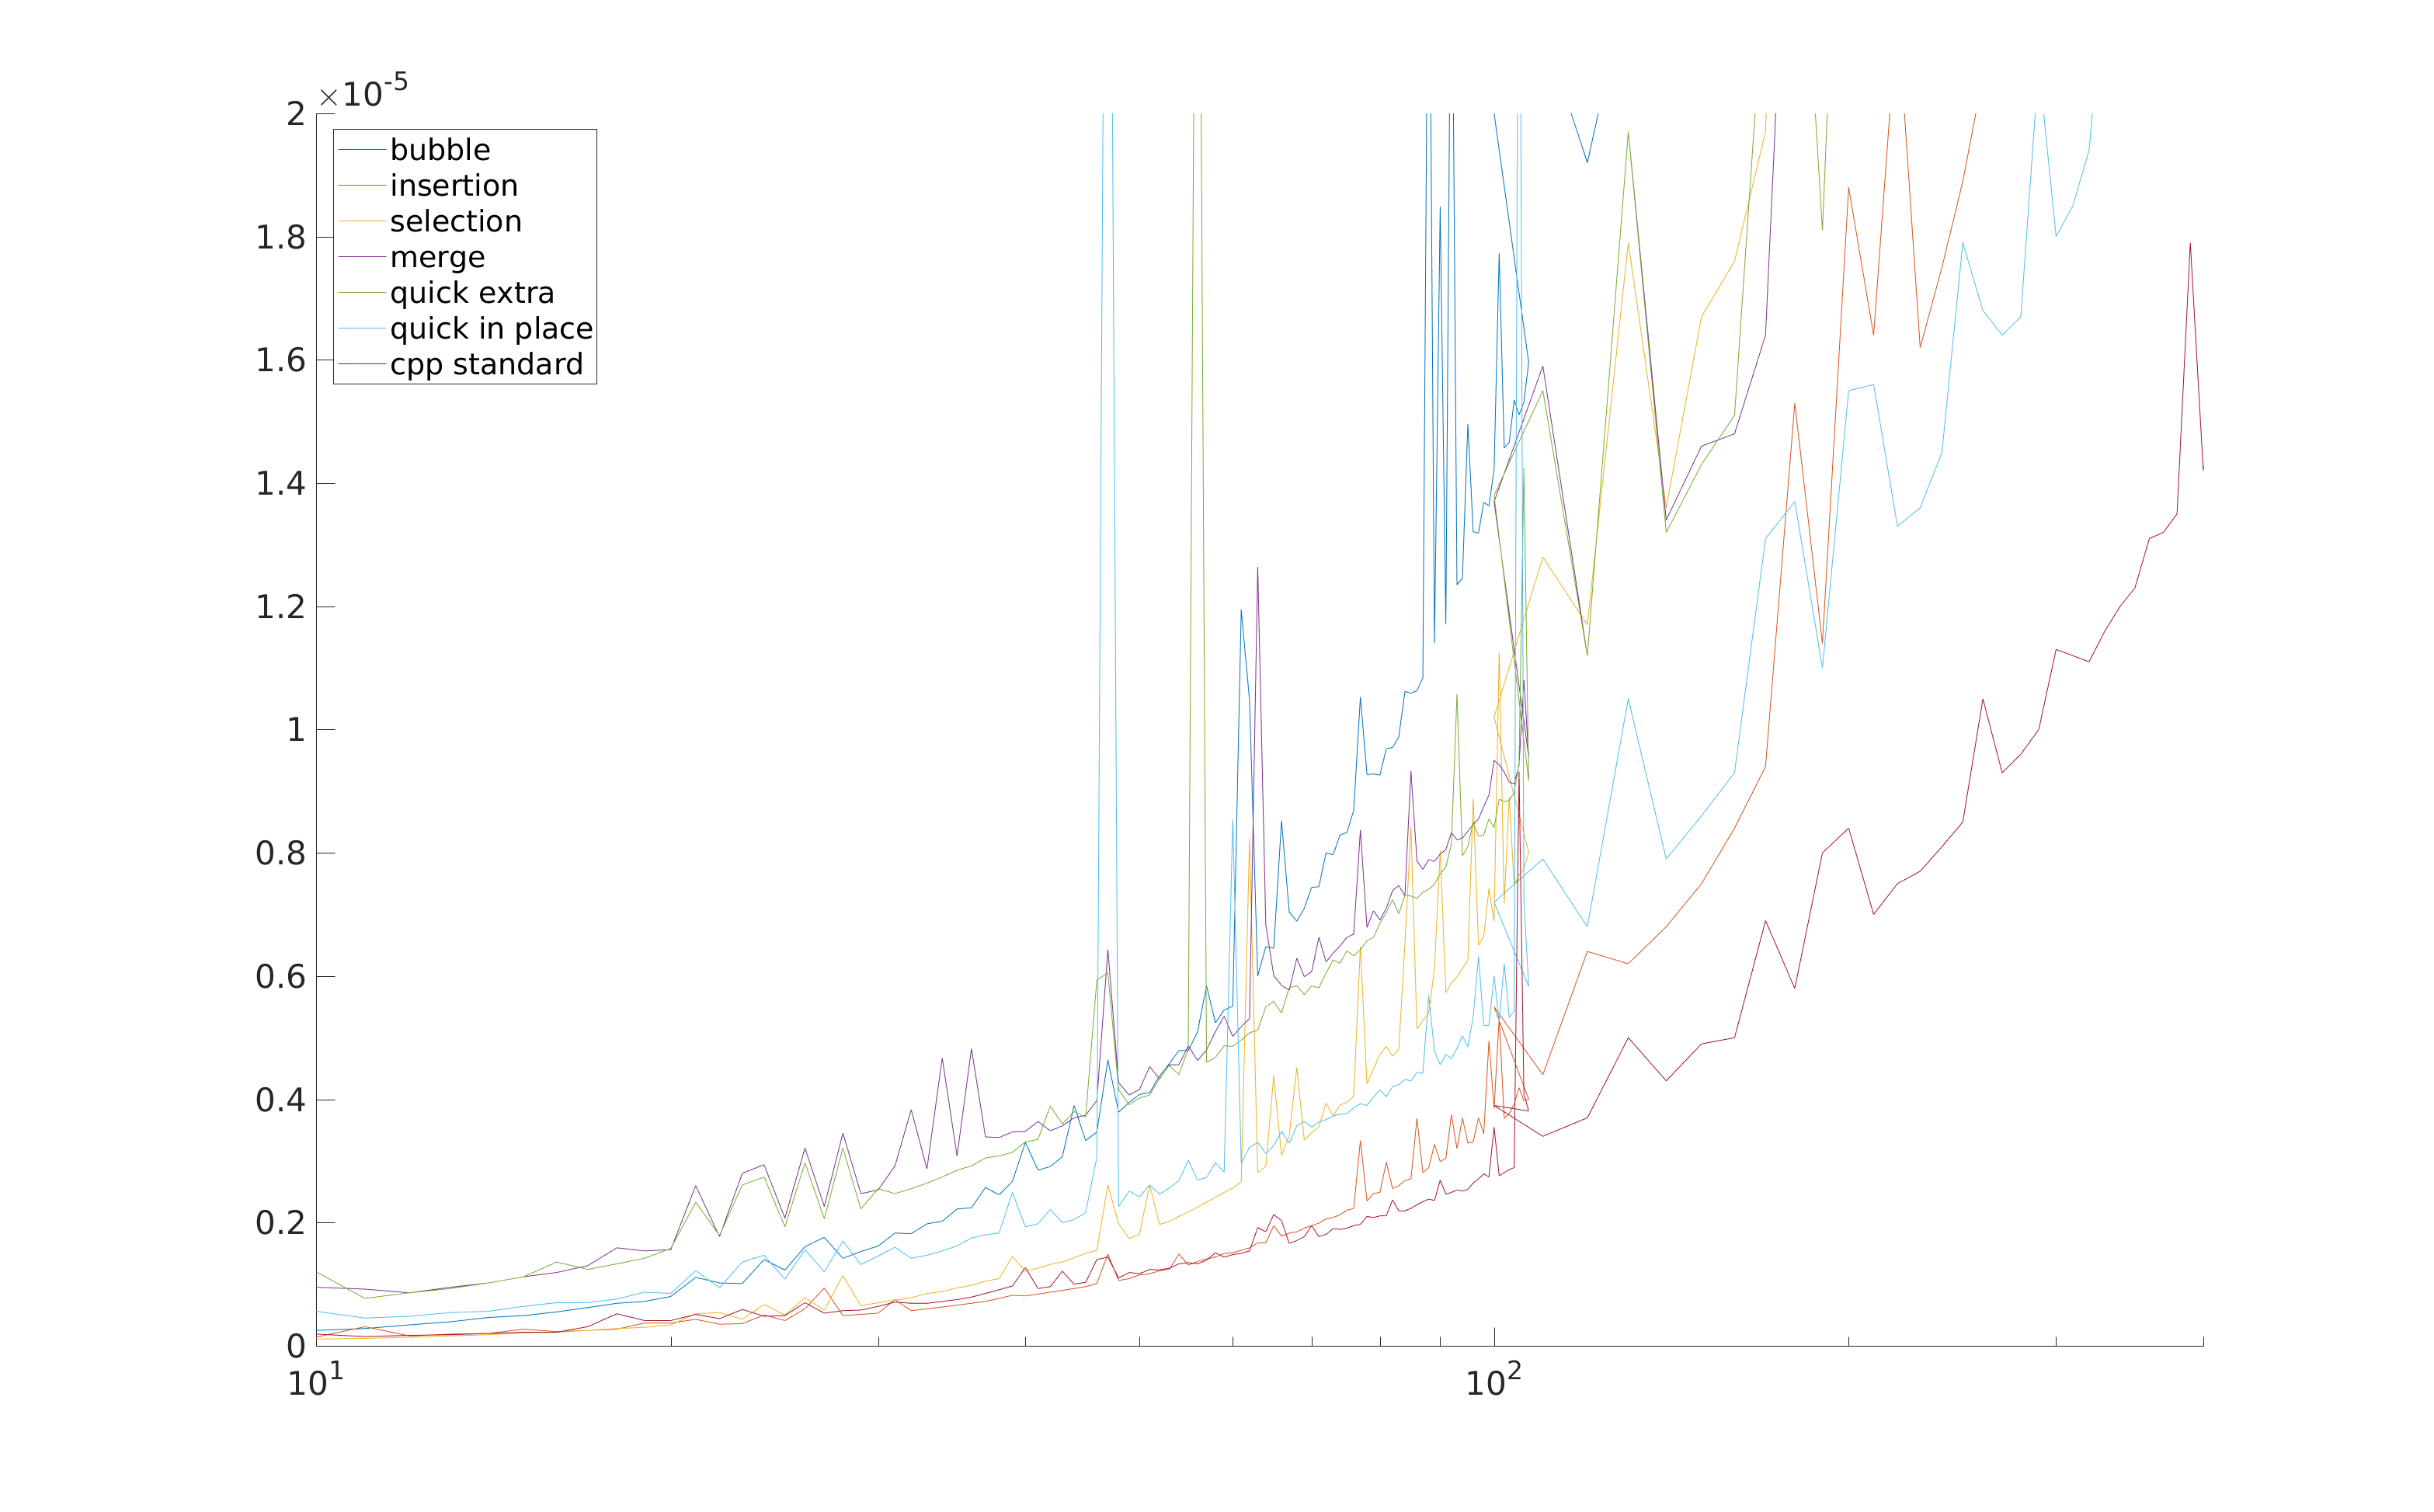
\includegraphics[width=0.8\linewidth]{../benchmark/fig2.png}
\caption{Small cases}
\label{fig-2}
\end{figure}

From Figure \ref{fig-2}, we can find that when the data size is small (from 10 to 100), the running speed of merge sort and quick sort is slower than insertion sort. It is because when $n$ is small, the constant $c$ acts a more important role. However, the cpp standard sort have a similar performance as insertion sort in this period, so it probably apply insertion sort to the data when $n$ is small enough. That's why the cpp standard sort is always quicker than my algorithms in Figure \ref{fig-1}.

\newpage

\section{Appendix}

\subsection{The project files}

\subsubsection{sort.h}
\inputminted{c++}{../answer/sort.h}
\subsubsection{sort.cpp}
\inputminted{c++}{../answer/sort.cpp}
\subsubsection{main.cpp}
\inputminted{c++}{../answer/main.cpp}
\subsubsection{Makefile}
\inputminted{makefile}{../answer/Makefile}


\subsection{The benchmark program}
\subsubsection{README.md}
\inputminted{md}{../benchmark/README.md}
\subsubsection{sort\_wrapper.h}
\inputminted{c++}{../benchmark/sort_wrapper.h}
\subsubsection{sort\_wrapper.cpp}
\inputminted{c++}{../benchmark/sort_wrapper.cpp}
\subsubsection{binding.gyp}
\inputminted{json}{../benchmark/binding.gyp}
\subsubsection{benchmark.js}
\inputminted{javascript}{../benchmark/benchmark.js}
\subsubsection{benchmark.m}
\inputminted{matlab}{../benchmark/benchmark.m}

\end{document}
